%%%%%%%%%%%%%%%%%%%%%%%%%%%%%%%%%%
\section{Results including photon transverse momentum}
%%%%%%%%%%%%%%%%%%%%%%%%%%%%%%%%%%
%------------------------------------------------------------------------------------
%\begin{table}

\begin{table}[tbp]
\begin{scriptsize}


\centering
\begin{tabular}{|c|c|c|c|}
\hline
contribution               &  $\sqrt{s}_{NN}$ = 8.16 TeV & $\sqrt{s}_{NN}$ = 8.16 TeV \\
\hline
  &  without cuts & $p_{T}>4 ~~GeV$, $|y|<2.4 $, $M_{l^+l^-}>10 ~~GeV$ \\

\hline
        LUX-like  F2+FL                 &      \\

$\gamma_{in} \gamma_{el}$  & 42.57    & 17.07\\

\hline
        LUX-like  F2                &       \\

$\gamma_{in} \gamma_{el}$  & 43.58   &  17.44\\


\hline
      ALLM97 F2          &   \\

      
$\gamma_{in} \gamma_{el}$  & 41.72    &16.43\\

\hline
      Fiore et al.\\(parametrization of JLAB data)    & \\

$\gamma_{in} \gamma_{el}$  & 45.24  &18.36\\
\hline
      SU F2      &        \\

      
$\gamma_{in} \gamma_{el}$  & 41.72   &16.70\\
\hline
      SY F2      &         \\

      
$\gamma_{in} \gamma_{el}$  & 40.38    &15.99\\

\hline
    Elastic- Elastic&               \\
$\gamma_{el} \gamma_{el}$   & 47,89  & 18.26  \\



\hline

\end{tabular}
\caption{Cross sections (in $n b$) for different contributions 
and different structure functions: LUX-like, ALLM97, Fiore, SU and SY.
(the cross section was scaled by factors: 0.96 (elastic-elastic); 0.95 (elastic-inelastic) for proton-ion absorption (multiple interactions))
}
\end{scriptsize}
\end{table}





%-----------------------------------------------------------------------------
\begin{figure}[!h]
\begin{minipage}{0.47\textwidth}
 \centerline{\includegraphics[width=1.0\textwidth]{figures_Marta/Mll.pdf}}
\end{minipage}
\begin{minipage}{0.47\textwidth}
 \centerline{\includegraphics[width=1.0\textwidth]{figures_Marta/Mll-c.pdf}}
\end{minipage}
\caption{The elastic - elastic and the inelastic-elastic contribution 
to dilepton invariant mass distributions 
for different structure functions. In the left panel we show the results for the whole phase space, while in the right panel only for the fiducial region.
}
 \label{fig:dsig_dMWW_ineine}
\end{figure}
%------------------------------------------------------------------------------

%-----------------------------------------------------------------------------
\begin{figure}[!htbp]
\begin{minipage}{0.47\textwidth}
 \centerline{\includegraphics[width=1.0\textwidth]{figures_Marta/pt1.pdf}}
\end{minipage}
\begin{minipage}{0.47\textwidth}
 \centerline{\includegraphics[width=1.0\textwidth]{figures_Marta/pt1-c.pdf}}
\end{minipage}
\caption{
Transverse momentum distribution of $\mu^+$ or $\mu^-$ 
for elastic - elastic and inelastic - elastic different structure functions: LUX-like, ALLM97, Fiore at all., SU and SY (in the left panel we show the results for the whole phase space, while in the right panel only for the fiducial region).
}
 \label{fig:dsig_dMWW_ineine}
\end{figure}
%------------------------------------------------------------------------------


%-----------------------------------------------------------------------------
\begin{figure}[!htbp]
\begin{minipage}{0.47\textwidth}
 \centerline{\includegraphics[width=1.0\textwidth]{figures_Marta/ptsum.pdf}}
\end{minipage}
\begin{minipage}{0.47\textwidth}
 \centerline{\includegraphics[width=1.0\textwidth]{figures_Marta/ptsum-c.pdf}}
\end{minipage}
\caption{
Distribution in transverse momentum of the $\mu^+ \mu^-$ pairs for elastic - elastic and 
inelastic-elastic
contributions
for different structure functions: LUX-like, ALLM97, Fiore at all., SU and SY. (in the left panel we show the results for the whole phase space, while in the right panel only for the fiducial region).
}
 \label{fig:dsig_dMWW_ineine}
\end{figure}
%------------------------------------------------------------------------------


%-----------------------------------------------------------------------------
\begin{figure}[!htbp]
\begin{minipage}{0.47\textwidth}
 \centerline{\includegraphics[width=1.0\textwidth]{figures_Marta/y1.pdf}}
\end{minipage}
\begin{minipage}{0.47\textwidth}
 \centerline{\includegraphics[width=1.0\textwidth]{figures_Marta/y1-c.pdf}}
\end{minipage}

\caption{
Rapidity distribution of $\mu^+$ or $\mu^-$ leptons
for elastic - elastic and inelastic-elastic contributions for different structure functions: LUX-like, ALLM97, Fiore at all., SU and SY. (in the left panel we show the results for the whole phase space, while in the right panel only for the fiducial region).
}
 \label{fig:dsig_dMWW_ineine}
\end{figure}
%------------------------------------------------------------------------------



%------------------------------------------------------------------------------

%-----------------------------------------------------------------------------
\begin{figure}[!htbp]
\begin{minipage}{0.47\textwidth}
 \centerline{\includegraphics[width=1.0\textwidth]{figures_Marta/MX.pdf}}
\end{minipage}
%\hspace{0.5cm}
\begin{minipage}{0.47\textwidth}
 \centerline{\includegraphics[width=1.0\textwidth]{figures_Marta/MX-c.pdf}}
\end{minipage}
\caption{
Missing mass distributions for eleastic-elastic photon-photon contributions and elastic-inelastic photon-photon contributions for different structure functions: LUX-like, ALLM97, Fiore at all., SU and SY. (in the left panel we show the results for the whole phase space, while in the right panel only for the fiducial region).
}
\label{fig:dsig_dy}
\end{figure}
%---------------------------------------------------------------




%-----------------------------------------------------------------------------
\begin{figure}[!htbp]
\begin{minipage}{0.47\textwidth}
 \centerline{\includegraphics[width=1.0\textwidth]{figures_Marta/ydiff.pdf}}
\end{minipage}
%\hspace{0.5cm}
\begin{minipage}{0.47\textwidth}
 \centerline{\includegraphics[width=1.0\textwidth]{figures_Marta/ydiff-c.pdf}}
\end{minipage}
\caption{
Distribution in rapidity distance between $\mu^+\mu^-$ leptons.
The calculation for the $\gamma-\gamma$ contribution
was performed for different structure functions. 
The left panel shows results  without cuts while the right panel 
shows results with ATLAS cuts.
}
\label{fig:dsig_dy}
\end{figure}
%---------------------------------------------------------------

%-----------------------------------------------------------------------------
\begin{figure}[!htbp]
\begin{minipage}{0.47\textwidth}
 \centerline{\includegraphics[width=1.0\textwidth]{figures_Marta/phi.pdf}}
\end{minipage}
%\hspace{0.5cm}
\begin{minipage}{0.47\textwidth}
 \centerline{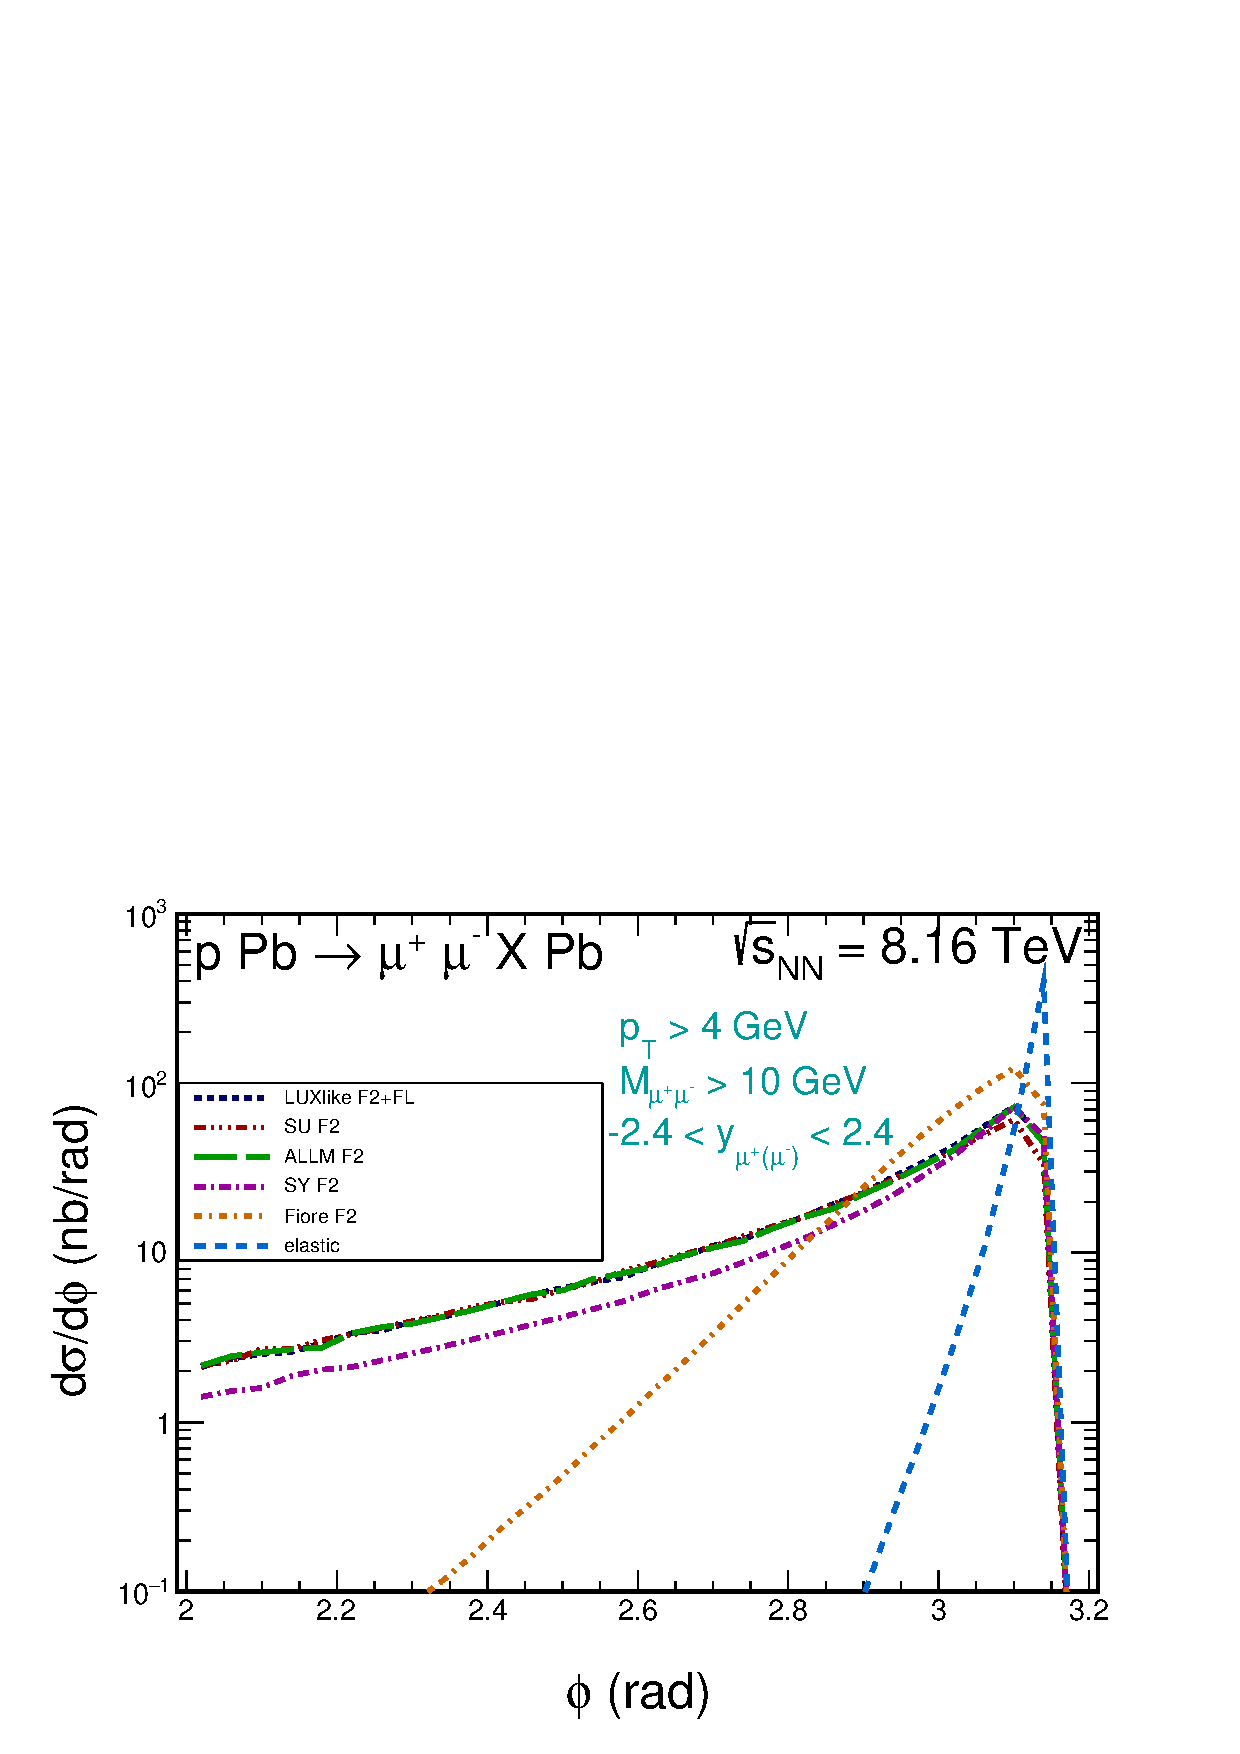
\includegraphics[width=1.0\textwidth]{figures_Marta/phi-c.pdf}}
\end{minipage}
\caption{
Distributions for azimuthal angle between $\mu^+\mu^-$ leptons. (in the left panel we show the results for the whole phase space, while in the right panel only for the fiducial region).
}
\label{fig:dsig_dy}
\end{figure}
%---------------------------------------------------------------




